\documentclass[a4paper,12pt]{article}

\title{Math 31 \\ Curve Sketching}
\author{Jad Chehimi}

% document setup
\renewcommand{\familydefault}{\sfdefault}
\linespread{1.25}
\usepackage[margin=1in]{geometry}
\usepackage{setspace}
\usepackage{enumitem}
\setlist{nosep}
\usepackage{color,soul}
\setcounter{secnumdepth}{0}

% tools
\usepackage[hidelinks]{hyperref}
\usepackage{float}
%% images
\usepackage{graphicx}
\graphicspath{ {./images/} }
%% science
\usepackage{siunitx}

\begin{document}
\maketitle

% temp
\begin{center}
\Huge
Unfinished!
\normalsize
\end{center}
% temp

\tableofcontents

\pagebreak

\section{Increasing and Decreasing Functions}
\begin{itemize}
    \item{If \hl{$f'(x) > 0$} for all values of $x$ in a range $(x_1, x_2)$,\\then $y = f(x)$ is \hl{increasing} in the range $(x_1, x_2)$}
    \item{If \hl{$f'(x) < 0$} for all values of $x$ in a range $(x_1, x_2)$,\\then $y = f(x)$ is \hl{decreasing} in the range $(x_1, x_2)$}
\end{itemize}

\section{Maxima and Minima}
\begin{itemize}
    \item{If \hl{$f(c) \geq f(x)$} for all values of $x$, then the \hl{maxima is $x = c$}}
    \item{If \hl{$f(c) \leq f(x)$} for all values of $x$, then the \hl{minima is $x = c$}}
\end{itemize}

\hl{Absolute} maxima/minima is for the \hl{entire domain} of $y = f(x)$

\hl{Local} maxima/minima is for the just the \hl{range of an interval} $(a, b)$

\subsection{Fermat's Theorem}
\textbf{Critical numbers} are points of a graph where a \hl{local min/max may occur}.

$f$ has a critical number at $x = c$ if either...
\begin{itemize}
    \item{$f'(c) = 0$\\(flat, horizontal portion of curve)}
    \item{$f'(c) = \textrm{DNE}$\\(divide by zero, e.g. cusp)}
\end{itemize}

\subsection{Find Absolute Max/Min of Continuous Function}
You can get the critical number(s) of a function by solving for $x$ when $f'$ equals zero.
\begin{itemize}
    \item{Find $f(x)$ at the critical numbers}
    \item{Only if within a closed interval $[a, b]$, \hl{find $f(a)$ and $f(b)$} (since you can't derive end points)}
    \item{The largest of these values is the absolute max, the smallest the absolute min}
\end{itemize}

\section{First Derivative Test}
\begin{itemize}
    \item{If $f'(x)$ changes from \hl{positive to negative} at $x=c$, then $f(c)$ is a local maxima}
    \item{If $f'(x)$ changes from \hl{negative to positive} at $x=c$, then $f(c)$ is a local minima}
    \item{If $f'(x)$ \hl{does not change sign} at $x=c$, then there is no max/min at $x=c$}
\end{itemize}

To find these things without a graphing calculator...
\begin{itemize}
    \item{Draw a number line with each critical number plotted}
    \item{\hl{Plug in any $x$ value} that is within the range \hl{between each critical number}, and take note of its \hl{sign}\\(you don't actually need $f(x)$ at the specific $x$, just the sign)}
    \item{Knowing the signs before and after a critical number will allow you to know if it is a local min or max}
\end{itemize}

\section{Max \& Min Applications}
\begin{itemize}
    \item{Find two equations that share variables}
    \item{
        Convert an equation with two variables into an equation with one
        \begin{itemize}
            \item{Choose any equation and isolate any variable to one side}
            \item{Substitute this new equation into the other}
        \end{itemize}
    }
    \item{Only now get the derivative of this equation}
    \item{Set it to equal $0$ and solve for \hl{either} variable}
    \item{Now that you have the missing information, do not forget to \hl{fulfill the rest of the question criteria}}
\end{itemize}

\begin{figure}[H]
    \centering
    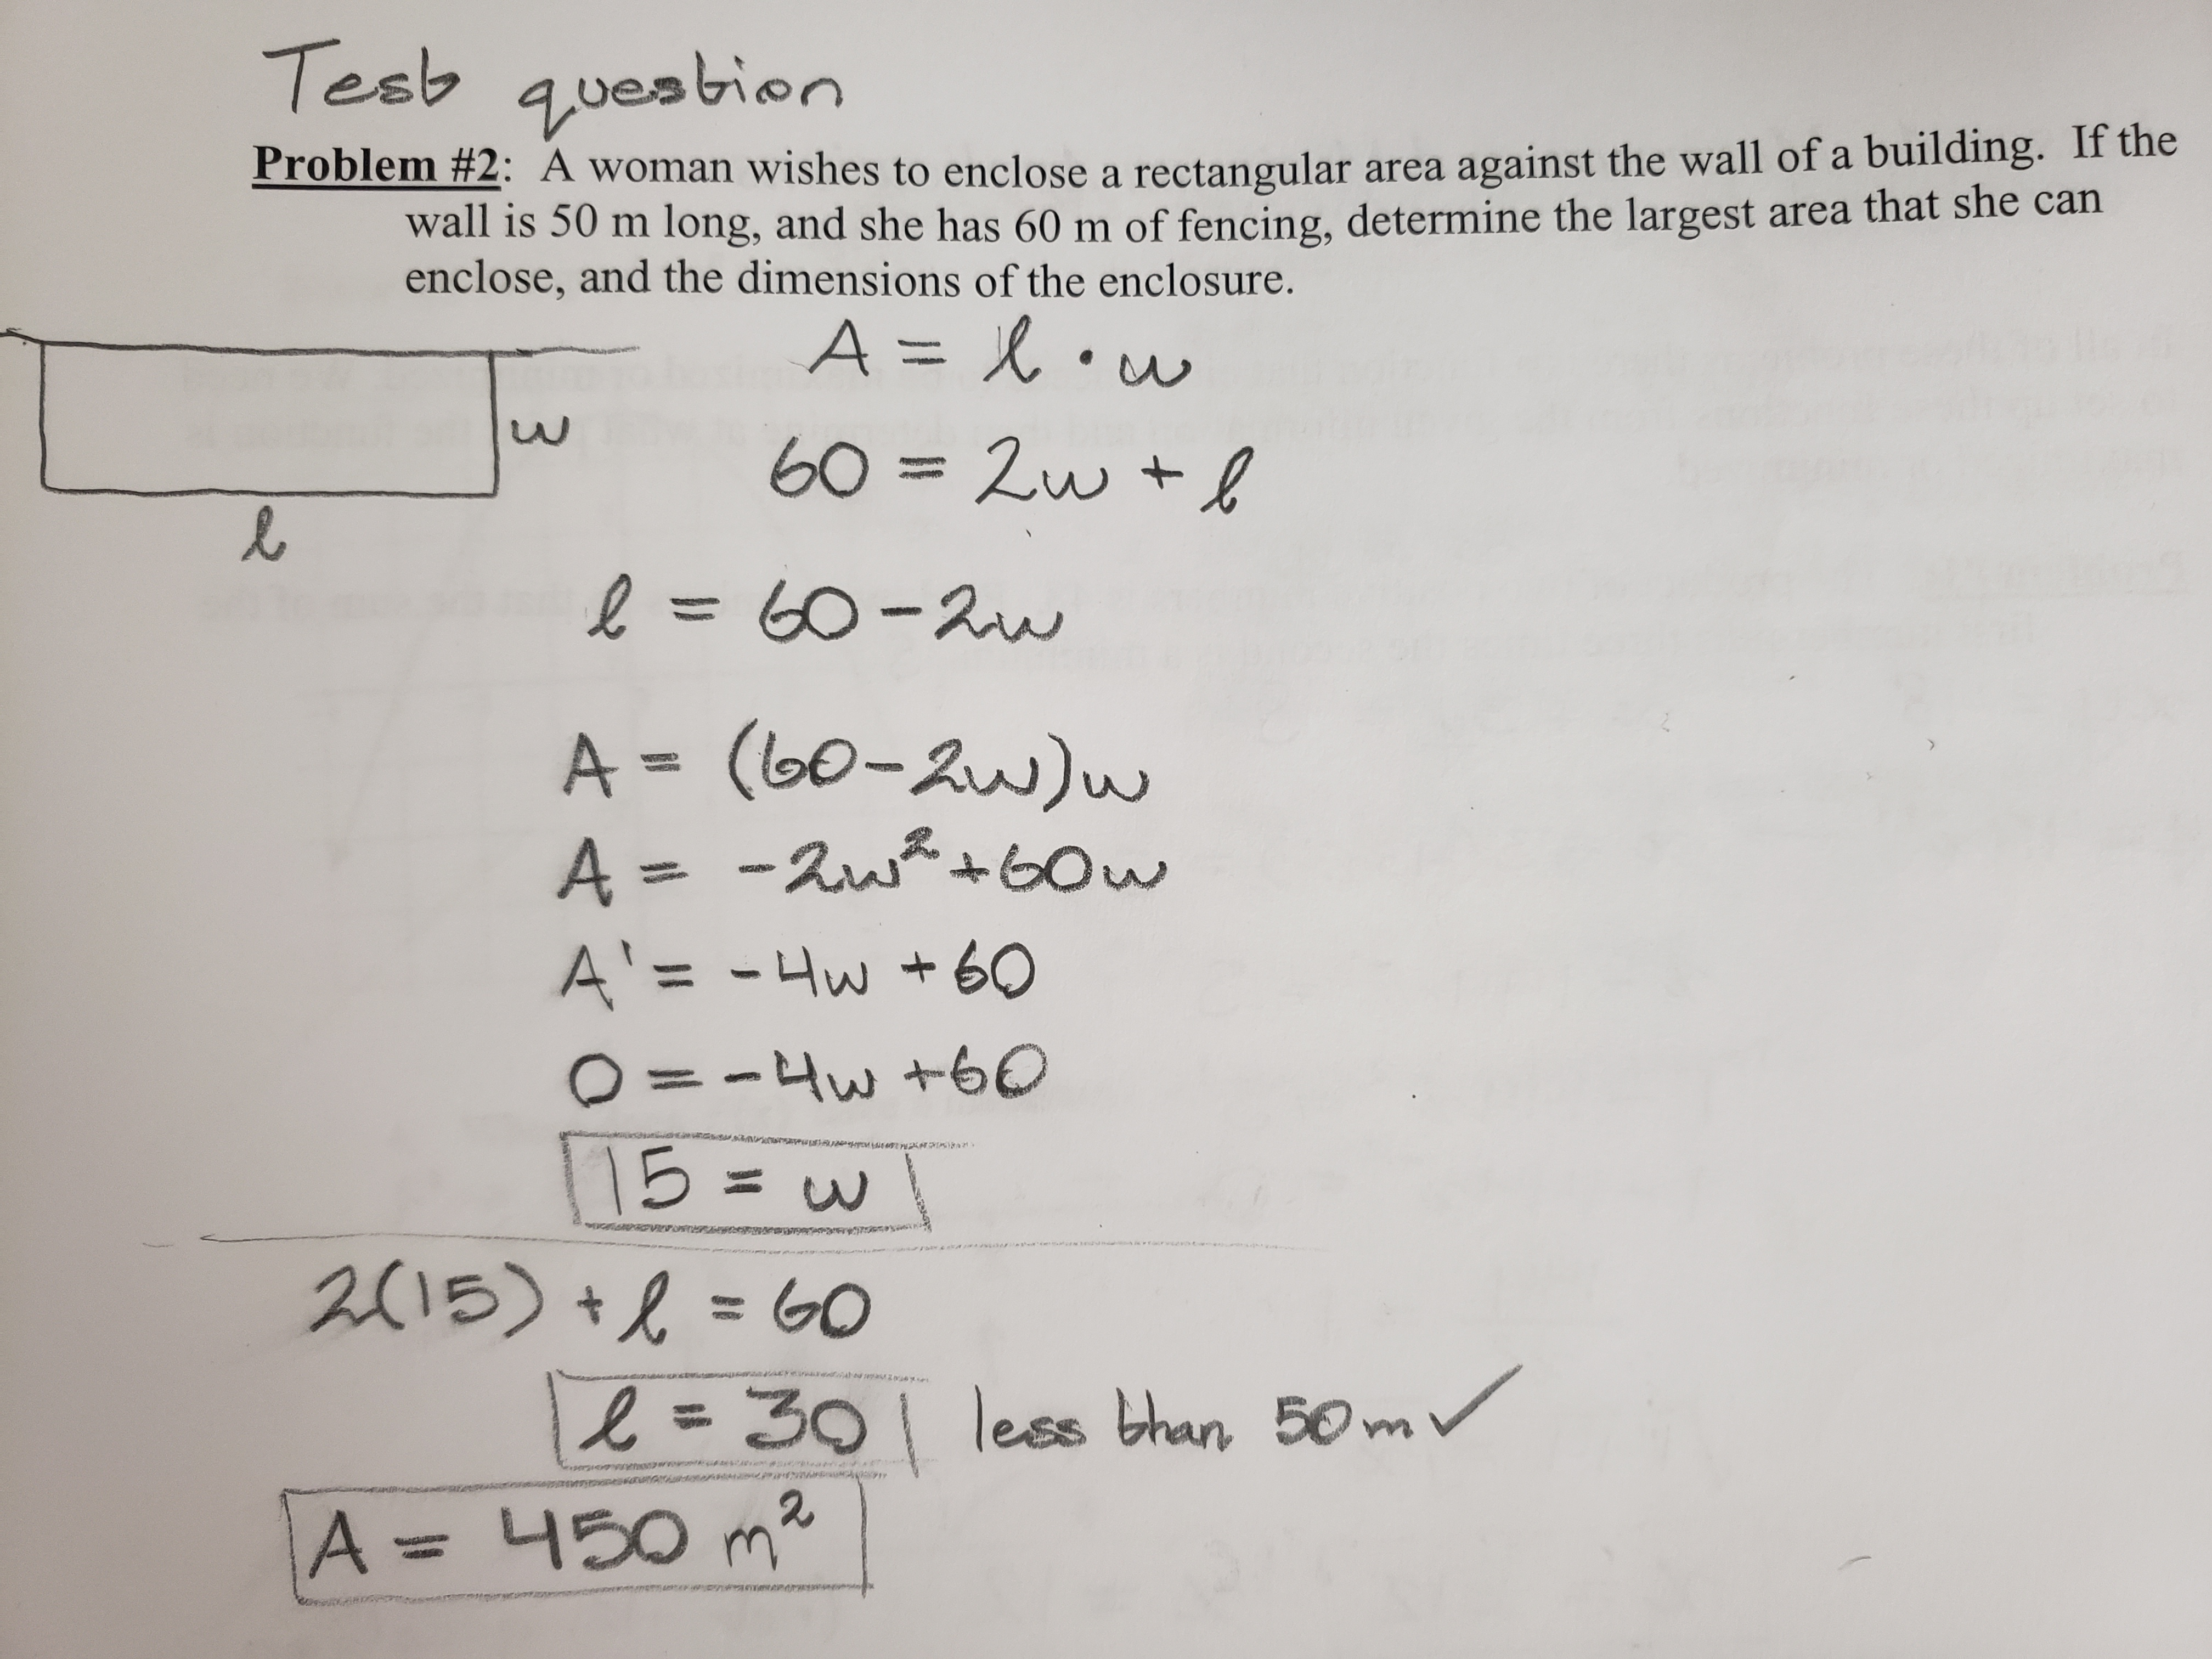
\includegraphics[width=\textwidth]{maxminapp}
\end{figure}

\section{Review}
\subsection{Domain}
The domain is all possible $x$ values of a function.
\begin{itemize}
    \item{Polynomial functions: all $x$ values valid}
    \item{Rational functions: any $x$ value that causes division by zero is invalid (NPV)}
    \item{Radical functions: any $x$ value that causes rooting negatives is invalid}
\end{itemize}

\subsection{Intercepts}
\begin{itemize}
    \item{\textbf{X-intercept}: $y = 0$, solve for $x$}
    \item{\textbf{Y-intercept}: $x = 0$, solve for $y$}
\end{itemize}

\section{Symmetry}
\begin{figure}[H]
    \centering
    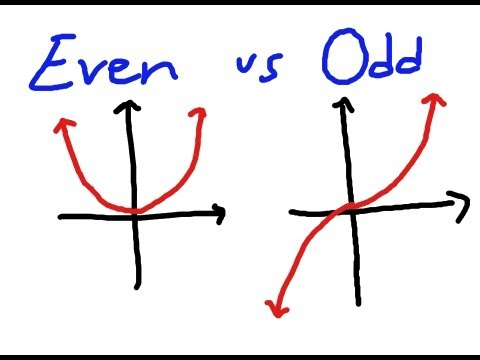
\includegraphics[width=0.50\textwidth]{evenodd}
\end{figure}
\subsection{Even Symmetry}
$$f(-x) = f(x)$$
If the above is true, then the function is has \textbf{even symmetry}.

Replace all instances of $x$ in the function with $-x$. 

If it makes \hl{no difference}, than it has even symmetry.

\subsection{Odd Symmetry}
$$f(-x) = -f(x)$$
If the above is true, then the function is has \textbf{odd symmetry}.

Replace all instances of $x$ in the function with $-x$. 

If the only difference is \hl{all signs flipped} (you could factor out $-1$) than it has odd symmetry.

\subsection{No Symmetry}
If the above two are both not true, then no symmetry is possible.

\section{Limits to Infinity of Asymptotes}
\subsection{Vertical}
$y = f(x)$ has a vertical asymptote of $x = a$ if...

\begin{center}
$\lim\limits_{x \to a^+} f(x) = \pm\infty$ \;\;\;or\;\;\; $\lim\limits_{x \to a^-} f(x) = \pm\infty$
\end{center}

The \hl{limit exists} even if left and right are \hl{different signs}, as long as its infinity.

\subsubsection{Determining Sign of Asymptote Limit}
Knowing whether an asymptote approaches positive or negative infinity is important when curve sketching.

\begin{itemize}
    \item{Find any vertical asymptotes (solve for $x$ when denominator = 0)}
    \item{Create two limits for $x$ approaching each vertical asymptote --- approaching from the left and right}
    \item{Factor denominator if possible (not required, but makes things easier)}
    \item{Determine the sign of limit by finding sign of numerator and denominator}
\end{itemize}

\subsubsection{Determine The Sign}
This is the hard part, since you don't really calculate anything.

\begin{itemize}
    \item{To test a limit of $x$ approaching the VA from the right, substitute all $x$ in the function with a value slightly larger than $x$ \\(e.g. if $\lim\limits_{x \to 2^+}$, then set something like $x = 2.1$)}
    \item{To test a limit of $x$ approaching the VA from the left, substitute all $x$ in the function with a value slightly smaller than $x$ \\(e.g. if $\lim\limits_{x \to 2^-}$, then set something like $x = 1.9$)}
\end{itemize}

e.g. Determine the vertical asymptote equation of $f(x) = \frac{1}{x}$.

Vertical asymptote is $x = 0$

$$\lim\limits_{x \to 0^+}\frac{1}{x} = \frac{1}{0.1} = \frac{+}{+} = +\infty$$
$$\lim\limits_{x \to 0^-}\frac{1}{x} = \frac{1}{-0.1} = \frac{+}{-} = -\infty$$

\pagebreak

\subsection{Horizontal}
This is the identical to "Finding Limits to Infinity" from Unit 1. It is the same for limits approaching positive or negative infinity.

\begin{itemize}
    \item{Any fraction with a variable to any power in the denominator will be zero. $$\lim\limits_{x\to\infty}{\frac{a}{x^b}} = 0$$}
    \item{Multiply a limit by something in order to put a variable (to the power of the highest existing power) under the terms, making them equal zero.}
\end{itemize}

$$\lim\limits_{x\to\infty}{\frac{6n+9}{3n-2}}$$
$$\frac{6n+9}{3n-2} \times \frac{\frac{1}{n}}{\frac{1}{n}}$$
$$\frac{6+\frac{9}{n}}{3-\frac{2}{n}} \longrightarrow \frac{6+0}{3-0}$$
$$\lim\limits_{x\to\infty}{\frac{6n+9}{3n-2}} = 2$$

\pagebreak

\section{Concavity}
\begin{figure}[H]
    \centering
    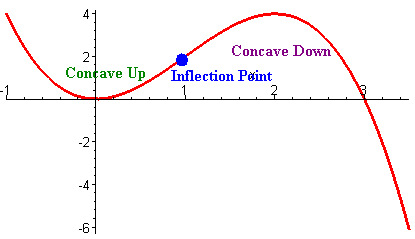
\includegraphics[width=0.50\textwidth]{concave}
\end{figure}

\subsection{Concave Up}
If the graph lies above the tangents of all of its points.

If \hl{$f''(x) > 0$} for all $x$ in an interval, $y = f(x)$ is \hl{concave upwards} in that interval.

\subsection{Concave Down}
If the graph lies below the tangents of all of its points.

If \hl{$f''(x) < 0$} for all $x$ in an interval, $y = f(x)$ is \hl{concave downwards} in that interval.

\subsection{Point of Inflection}
If $f''(x)$ \hl{changes sign} (+ to -, - to +) at $x = c$, then a \textbf{point of inflection} occurs at $x = c$.

\section{Second Derivative Test}
\begin{itemize}
    \item{If $f'(c) = 0$ AND $f''(c) < 0$, then the local max is at $x = c$}
    \item{If $f'(c) = 0$ AND $f''(c) > 0$, then the local min is at $x = c$}
\end{itemize}

\end{document}
